\chapter{Zero-dimensional laser-sustained plasma model} \label{chp:models}

    To predict experimental data, namely the pressure increase of the gas that should be expected when laser energy is input, the heat capacity of argon and hydrogen was modelled. A zero-dimensional (0D) heat transfer model was then written in Python to compare to experimental data. Argon and hydrogen were used to validate initial equilibrium calculations, while the 0D model was solely implemented using argon. Argon was the main gas used in experiments, as it was economical and easy to ionize. Hydrogen is projected to be used in a full-scale LTP engine for its increased $I_\mathrm{sp}$ due to its lower molecular weight.

    \section{Equilibrium calculations} \label{sec:equilibrium calcs}
        
        The following seventh order polynomials and their coefficients ($a_1$ to $a_7$, $b_1$, and $b_2$), from \textcite{mcbrideNASAGlennCoefficients2002}, were implemented in Python. Species of interest were \ce{H}, \ce{H2}, \ce{Ar}, \ce{Ar+}, and electrons \ce{e-}. Plasma temperatures studied allowed us to treat the argon as singly ionized, and the hydrogen as dissociated. The heat capacity at constant pressure, as well as the temperature ($T$) dependent part of enthalpy and entropy of each species are given by $c_p^0$, $h^0$, and $s^0$, respectively. $\bar R$ is the universal gas constant.

        \begin{equation}
            c_p^0 (T)/\bar R = a_1 T^{-2} + a_2 T^{-1} + a_3 + a_4   T + a_5 T^2 + a_6 T^3 + a_7 T^4
        \end{equation} 
        
        \begin{equation}
            h^0 (T)/\bar RT = -a_1 T^{-2} + a_2 \ln(T)/T + a_3 + a_4 T / 2 + a_5 {T^2}/3 + a_6 {T^3}/4 + a_7 {T^4}/5 + b_1/T
        \end{equation}
        
        \begin{equation}
            s^0(T)/\bar R = -a_1 T^{-2}/2 - a_2 T^{-1} + a_3\ln(T) + a_4   T + a_5 {T^2}/2 + a_6 T^3/3 + a_7 T^4/4 + b_2
        \end{equation}

        Next, the functions for entropy $\bar s_i$ of each species $i$ and Gibbs energy $\bar g_i$, both per \unit{kmol}, were implemented. These values depend on temperature $T$ and partial pressure $p_i$. $y_i$ is the molar fraction of the species, and $p_\mathrm{ref}$ is the reference pressure, equal to \qty{1}{bar}.
        
        \begin{equation}
            \bar s_i (T, p_i) = \bar s_i^0 (T) - \bar R \ln \frac{y_i p}{p_\mathrm{ref}}
        \end{equation}

        \begin{equation}
            \bar g_i = \bar h_i - T \bar s_i
        \end{equation}

        Considering the number of moles $n_i$, expressions of the Gibbs energy of the two mixtures $G_\mathrm{mixture}$ were found:

        Starting with \qty{1}{kmol} argon,
        \begin{equation}
            G_\mathrm{mixture,\: Ar}(T, p) = n_\mathrm{Ar} \bar g_\mathrm{Ar}(T, p_\mathrm{Ar}) + n_\mathrm{Ar+} \bar g_\mathrm{Ar+}(T, p_\mathrm{Ar+}) + n_\mathrm{e} \bar g_\mathrm{e}(T, p_\mathrm{e})
        \end{equation}

        Starting with \qty{1}{kmol} hydrogen,
        \begin{equation}
            G_\mathrm{mixture,\: H_2}(T, p) = n_\mathrm{H} \bar g_\mathrm{H}(T, p_H) + n_\mathrm{H2} \bar g_\mathrm{H2}(T, p_\mathrm{H2})
        \end{equation}

        \autoref{fig:Gibbs} plots the Gibbs energy of the hydrogen mixture as a function of its degree of dissociation $x$, for different total pressures $p$.

        \begin{figure}[!ht]
            \centering
            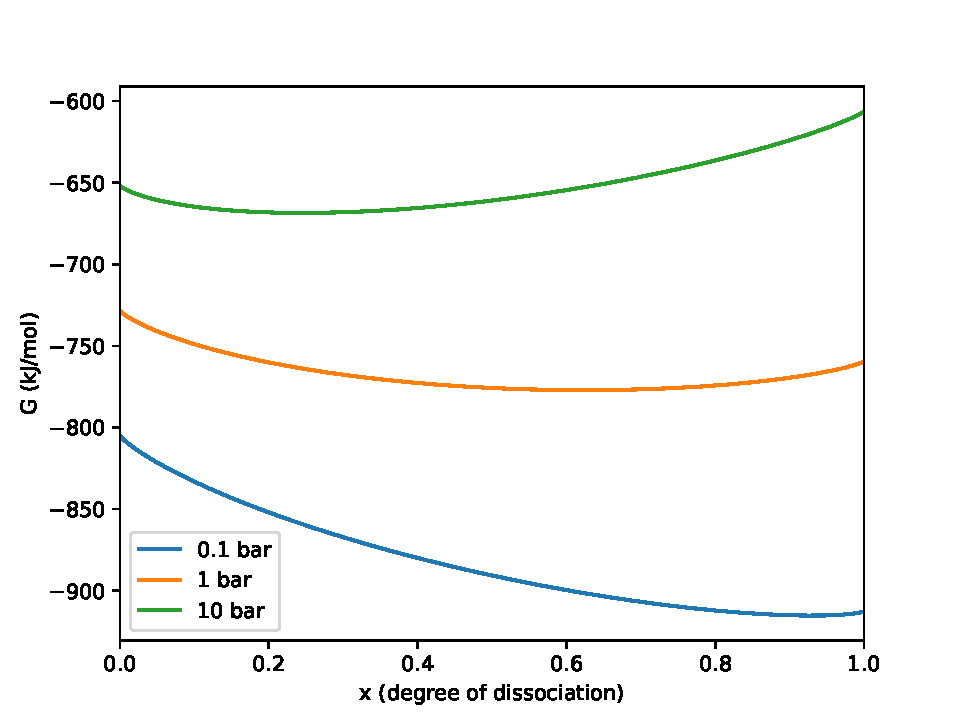
\includegraphics[width=0.7\textwidth]{assets/2 models/Gibbs.pdf}
            \caption{Gibbs free energy ($G$) plotted against the degree of dissociation ($x$) of hydrogen under three different pressures}
            \label{fig:Gibbs}
        \end{figure}

        A similar dissociation graph can be found with argon, but with three species. The Gibbs energy was then minimized to determine the molar fractions $y_i$ at which the mixture reaches equilibrium. From this, the enthalpy $H$ of the mixture was found. The $c_p$ of the mixture was then calculated from the enthalpy with:

        \begin{equation}
            c_p = \frac{\partial h}{\partial T}\bigg|_{p = const.}
        \end{equation}
        
        For argon, these calculated $c_p$ values were validated against values from CEA \cite{CEARUNRev4} in \autoref{fig:Cp_compare}.
        
        \begin{figure}[!ht]
            \centering
            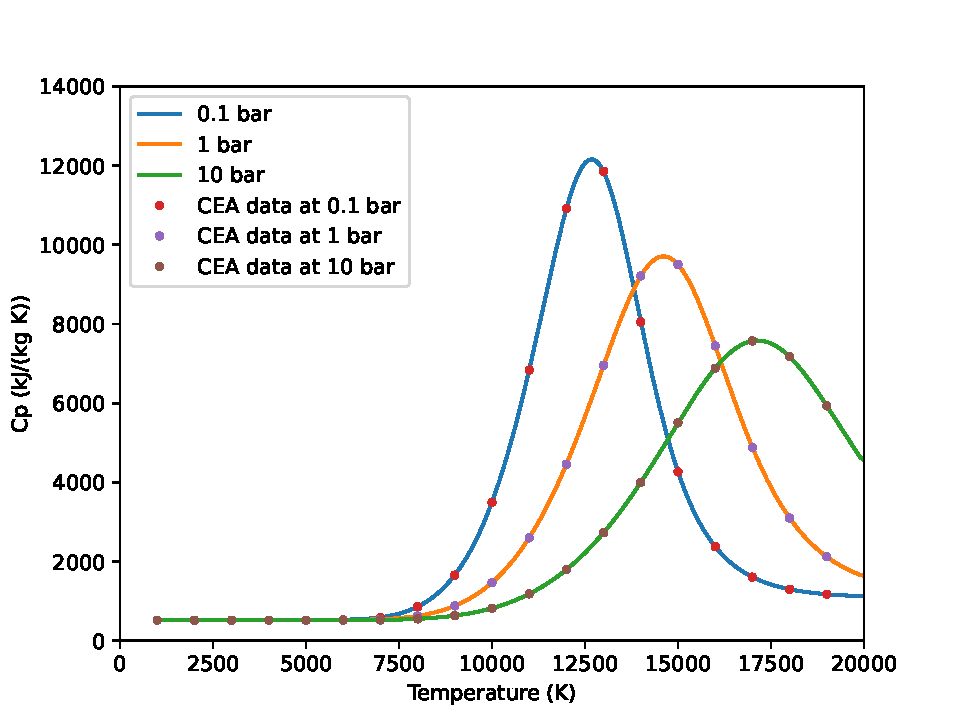
\includegraphics[width=0.7\textwidth]{assets/2 models/Cp_compare.pdf}
            \caption{Comparing calculated $c_p$ values of argon to those from CEA}
            \label{fig:Cp_compare}
        \end{figure}

        The properties of the argon plasma will be used as the basis of the 0D LSP model.
    
    \section{Bremsstrahlung energy loss}
        
        The main source of radiation found in LSP is Bremsstrahlung, or braking radiation. When an electron passes close to a heavier ion, it is deflected by the ion's electric field. This collision releases a photon \autocite{glasstoneControlledThermonuclearReactions1975}. The total radiated power density $P_\mathrm{br}/V$ of the collisions can be estimated with the formulas presented in \autoref{tab:Brems_compare}.

        \begin{table}[!ht]
            \footnotesize
            \centering
            \caption{Comparison of Bremsstrahlung power density loss}
            \label{tab:Brems_compare}
            \begin{tabularx}{\textwidth}{@{}lX<{\raggedright}@{}X<{\raggedright}@{}}
            \toprule
            Reference & Formula & SI Conversion \\ \midrule
            \textcite{glasstoneControlledThermonuclearReactions1975}  & $P_\mathrm{br}/V = 1.57 \times 10^{-27} n_\mathrm{e} n_\mathrm{i} Z^2 T^{1/2}$ \: $\mathrm{ergs/(cm^3\cdot s)}$, with T in K. &   $P_\mathrm{br}/V = 1.57 \times 10^{-28} n_\mathrm{e} n_\mathrm{i} Z^2 T^{1/2}$ \: $\mathrm{W/m^3}$  \\
            \textcite{rybickiRadiativeProcessesAstrophysics2004}      & $P_\mathrm{br}/V = 1.4 \times 10^{-27} n_\mathrm{e} n_\mathrm{i} Z^2 T^{1/2} \bar{g}_\mathrm{B}$ \: $\mathrm{ergs/(cm^3\cdot s)}$, with T in K.&  $P_\mathrm{br}/V = 1.68 \times 10^{-28} n_\mathrm{e} n_\mathrm{i} Z^2 T^{1/2}$ \:  $\mathrm{W/m^3}$, using $\bar{g}_\mathrm{B} (T)$ = 1.2\\
            \bottomrule          
            \end{tabularx}
        \end{table}

        The first relation, from \textcite{glasstoneControlledThermonuclearReactions1975} converted to SI, was used for the remainder of the calculations.

        There was also a question regarding whether this plasma was a surface emitter or a volume emitter. This was determined by calculating the plasma frequency at a typical electron density and comparing it to the wavelength of the light emitted by Bremsstrahlung. If the plasma frequency was higher than the wavelength of emitted Bremsstrahlung light, then it was cut off by the plasma; no light could escape directly from the inside of the LSP cone, and it was a surface emitter. If it was lower, then the emitted photons were not blocked by the LSP and the cone was a volumetric emitter.
        
        The plasma frequency $\omega_\mathrm{p}$ was found with: 

        \begin{equation}
            \omega_\mathrm{p} = \sqrt{\frac{n_\mathrm{e} e^2}{\epsilon_\mathrm{0} m_\mathrm{e}}}
        \end{equation}

        With $n_\mathrm{e}$ the plasma electron density, $e$ the elementary charge, $\epsilon_\mathrm{0}$ the vacuum permittivity, and $m_\mathrm{e}$ the electron mass.

        In the worst case scenario (highest temperature and pressure) of \qty{20000}{K} and \qty{20}{bar}, an electron density of \num{3.05e21} was found. This resulted in $\omega_p =$ \qty{3.11e12}{Hz}. Considering visible light and above (> \qty{1e14}{Hz}) as the wavelengths of interest, the LSP was indeed a volume emitter.

    \section{Model setup}
        
        Finally, a 0D model was written in Python to attempt to explain the pressure rise seen in the LTP experiments. \autoref{fig:0D model} illustrates this model. Laser energy is focused into a volume of argon, creating an LSP cone. Energy is transferred from the LSP cone to the larger argon volume by Bremsstrahlung. A part of the laser energy is also transmitted through the cone to the outside of the argon volume and lost, but this was not modelled. The LSP was treated as an ideal gas.

        \begin{figure}[!ht]
            \centering
            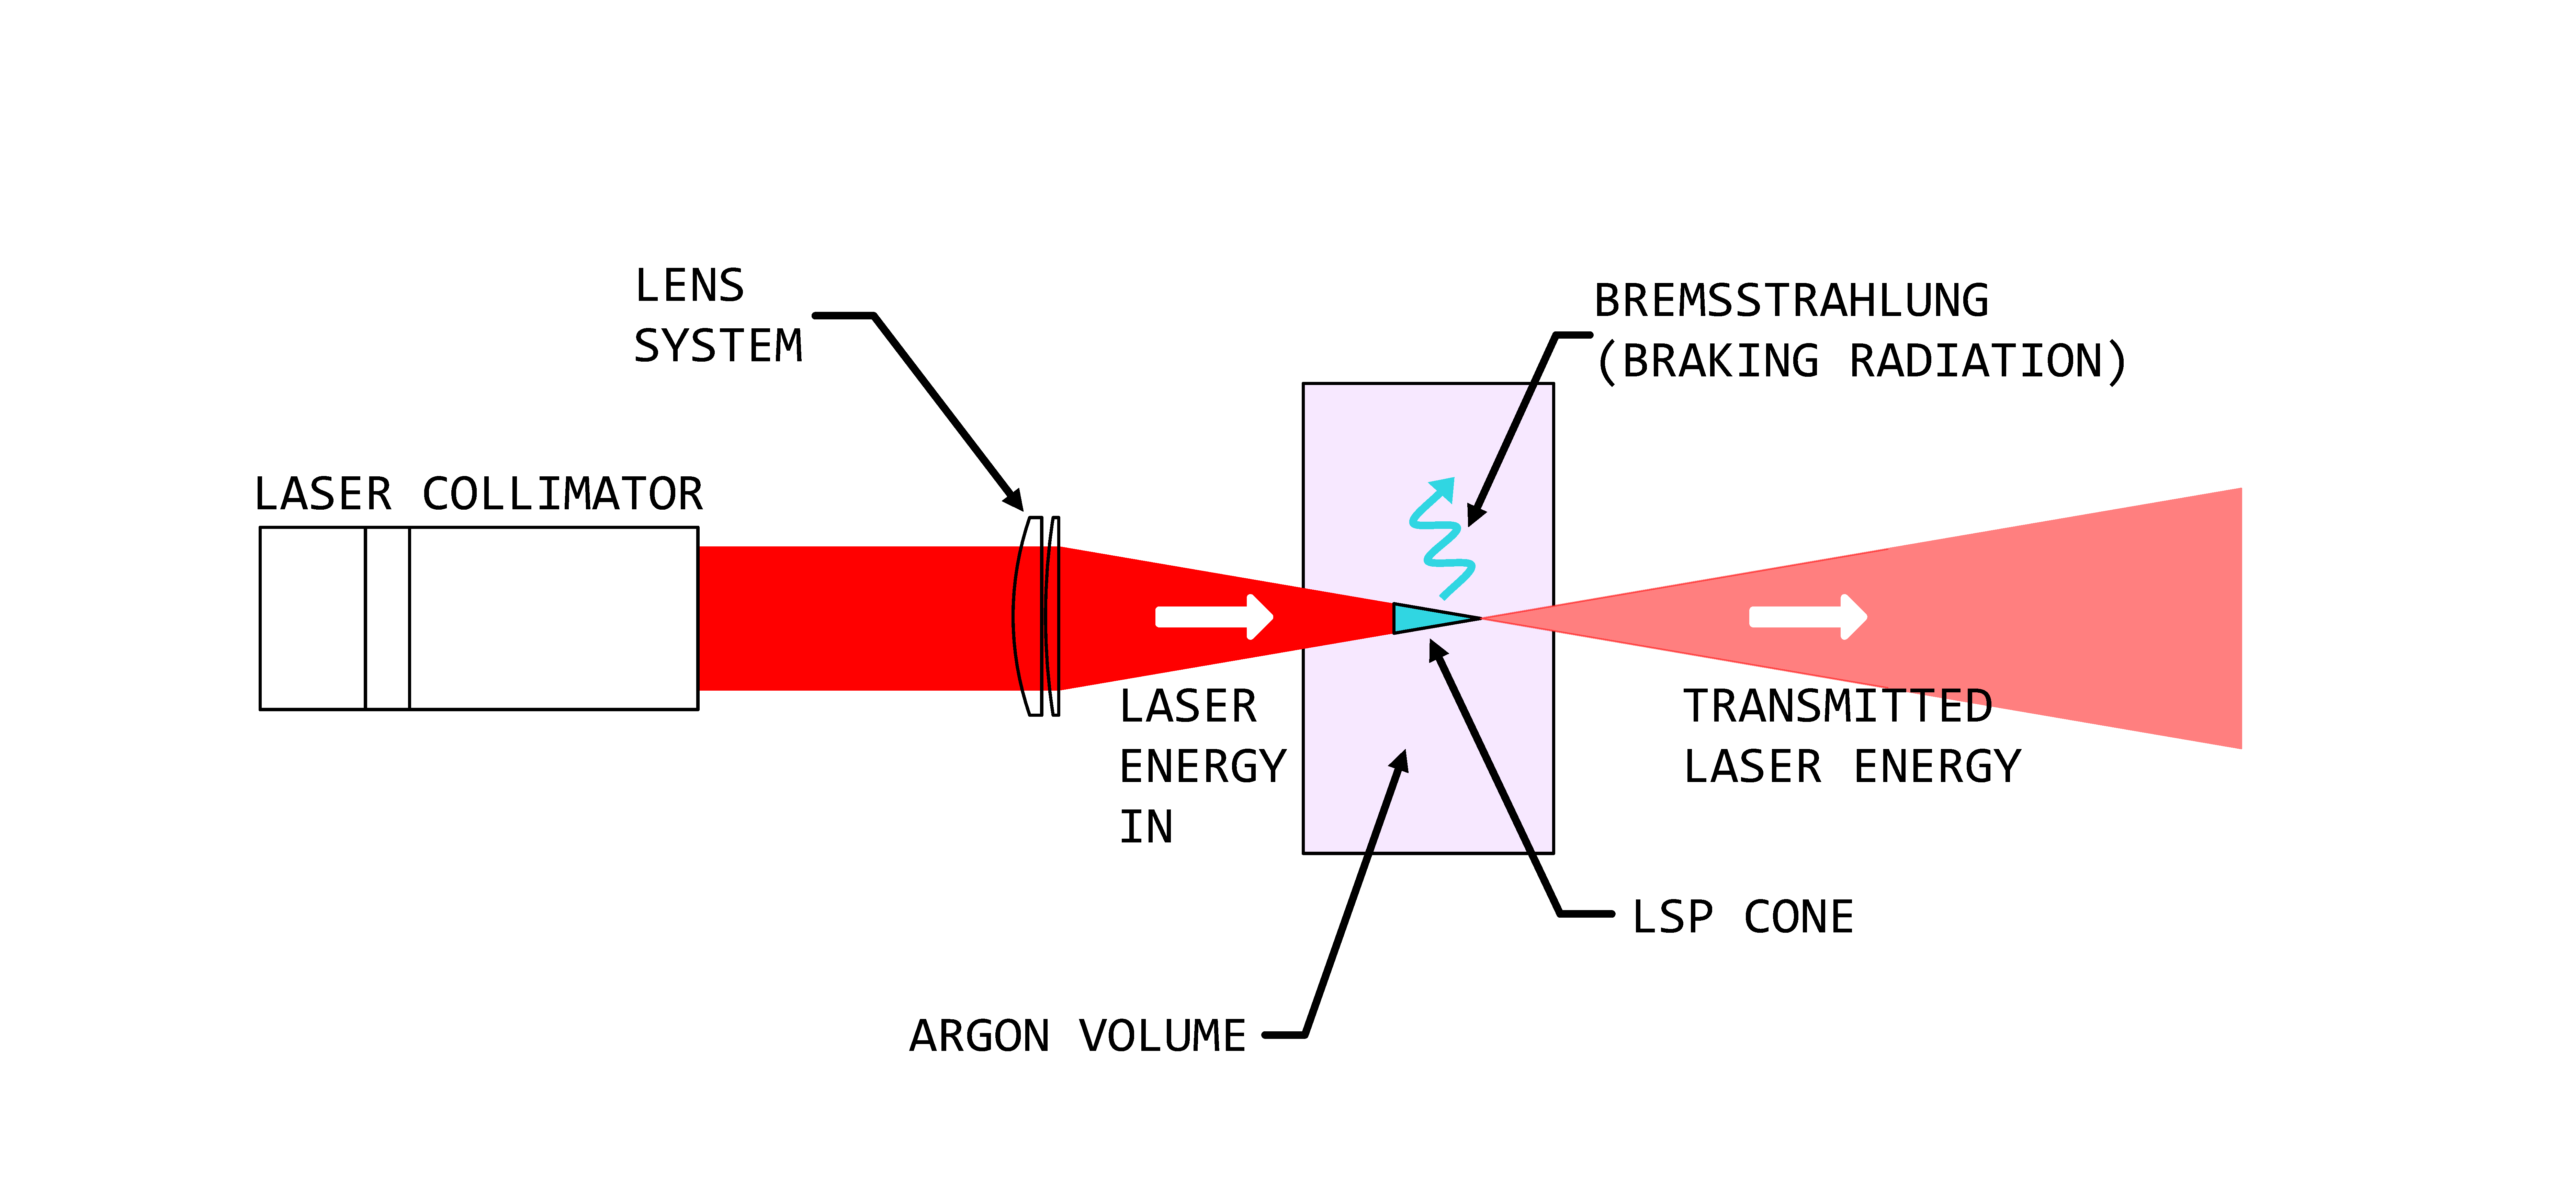
\includegraphics[width=0.85\textwidth]{assets/2 models/Modeling figure.pdf}
            \caption{Model of an LSP inside a volume of pressurized argon}
            \label{fig:0D model}
        \end{figure}

        The calculation procedure implemented in the 0D model was as follows:

        \begin{enumerate}
            \item The volume $V_\mathrm{plasma}$ and the mass $m_\mathrm{plasma}$ of a cone of pure argon were found at the initial temperature ($T_\mathrm{ini} = \qty{300}{K}$) and pressure ($p_\mathrm{ini} \approx \qty{20}{bar}$, set to the experimental measurement done before each shot). This was the mass of argon plasma and will remain fixed for the rest of the problem. This fixed mass could be a source of error, as the plasma propagates as described in \autoref{fig:Mechanism of LSP growth}. The length ($l_\mathrm{plasma}$) and radius ($r_\mathrm{plasma}$) of the plasma cone were taken from previous observations in \textcite{duplayArgonLaserPlasmaThruster2024a} when the cone reached equilibrium near the end of a laser pulse. The argon volume contained in the V1 test section was \qty{0.4}{L}.
                \begin{equation}
                    l_\mathrm{plasma} = \qty{0.02}{m}, \: r_\mathrm{plasma} = \qty{0.001}{m}
                \end{equation}
                \begin{equation}
                    V_\mathrm{plasma} = \frac{\pi r_\mathrm{plasma}^2}{3}
                \end{equation}
                \begin{equation}
                    m_\mathrm{plasma} = V_\mathrm{plasma}\rho(T_\mathrm{ini}, p_\mathrm{ini})
                \end{equation}
            \item The energy in the plasma $E_\mathrm{plasma}$ was calculated, starting at \qty{0}{J}. Energy from the laser pulse was added to the cone while the energy lost from radiation, calculated at the previous iteration, was subtracted. These were calculated from their respective powers $P$.
                \begin{equation}
                    E_\mathrm{plasma} = E_\mathrm{plasma} + \underbrace{P_\mathrm{laser} \times \mathrm{timestep}}_\textrm{Energy from the laser pulse} - \underbrace{P_\mathrm{loss} \times \mathrm{timestep}}_\textrm{Energy lost by radiation}
                \end{equation}
                The new temperature ($T_2$) of the cone at this step was found at constant pressure,
                \begin{equation}
                    E_\mathrm{plasma} = m_\mathrm{plasma} \left(h_2 (T_2, p_\mathrm{ini}) - h_1(T_\mathrm{ini}, p_\mathrm{ini})\right)
                \end{equation}
                where this equation was solved for $T_2$. The enthalpy of the argon was found with the relations implemented in \autoref{sec:equilibrium calcs}.
            \item The number of moles $n$ in the cone was found by minimizing the Gibbs free energy (see again \autoref{sec:equilibrium calcs}) at the temperature and pressure of step 2 ($T_2, p_2$). This gave the ionization fraction $x$.
                \begin{equation}
                    n = \frac{m_\mathrm{plasma}}{M_\mathrm{Ar}}(x + 1)
                \end{equation}
                The atomic mass of argon is $M_\mathrm{Ar} = \qty{39.948}{u}$. The new volume of the cone ($V_2$) was then found with the ideal gas law.
                \begin{equation}
                    V_2 = \frac{n \bar{R} T_2}{p_2}
                \end{equation}
                With the universal gas constant $\bar{R}$.
            \item The pressure increase $p_4$ of the larger argon volume in the V1 chamber (\qty{0.4}{L}) due to the isentropic expansion of the gas in the LSP cone was calculated.
                \begin{equation}
                    p_4 = p_\mathrm{ini} \left(\frac{V_\mathrm{chamber} - V_\mathrm{plasma}}{V_\mathrm{chamber} - V_2}\right)^\gamma
                \end{equation}
                With $\gamma=1.67$, the heat capacity ratio of argon at \qty{300}{K}. $p_2$ was set equal to $p_4$ at this point, so that the LSP cone would be at the same pressure as the surrounding gas for the next iteration.
            \item The radiated power from the LSP cone to the larger argon volume was determined for the next iteration. The Bremsstrahlung power density loss equation from \textcite{glasstoneControlledThermonuclearReactions1975} was used, multiplied by the volume $V_2$ of the LSP.
                \begin{equation}
                    P_\mathrm{br} = 1.57 \times 10^{-28} n_\mathrm{e} n_\mathrm{i} Z^2 T_2^{1/2} V_2
                \end{equation}
                With $Z = 1$, as the argon was singly ionized.
            \item Steps 2 to 5 were looped until \qty{10}{ms}, when laser energy deposition ended. No more energy was added but Bremsstrahlung loss continued. The conservation of energy equation thus became:
                \begin{equation}
                    E_\mathrm{plasma} = E_\mathrm{plasma} - P_\mathrm{loss} \times \mathrm{timestep}
                \end{equation}
        \end{enumerate}
        
        To determine an upper bound for power loss, a switch was implemented to change Bremss-trahlung loss to blackbody radiation loss. This would be the case if the LSP was a surface emitter. The power loss was computed by first finding the area of the cone $A_\mathrm{plasma}$. The length was found from the volume of the cone (which is known), while the radius was considered fixed at $r_\mathrm{plasma, fixed} = \qty{0.001}{m}$.
        \begin{equation}
            l_\mathrm{plasma} = \frac{3 V_\mathrm{plasma}}{\pi r_\mathrm{plasma, fixed}^2}
        \end{equation}
        The area of the cone and the power loss are then found. 
        \begin{equation}
            A_\mathrm{plasma} = \pi r_\mathrm{plasma, fixed} ( r_\mathrm{plasma, fixed} + \sqrt{l_\mathrm{plasma}^2 + r_\mathrm{plasma, fixed}^2})
        \end{equation}
        \begin{equation}
            P_\mathrm{loss} = \sigma T_2^4 A_\mathrm{plasma}
        \end{equation}
        With the Stefan-Boltzmann constant $\sigma$.
    \section{Model results}

        From these iterations, pressure rise curves with Bremsstrahlung loss and blackbody radiation loss were determined. These curves were overlaid on experimental data from LSP178\_SPRK49, a \qty{10}{ms} QCW LSP experiment at \qty{3079}{W} and \qty{19.91}{bar} of argon to give \autoref{fig:LSP178_SPRK49}.
        
        \begin{figure}[!ht]
            \centering
            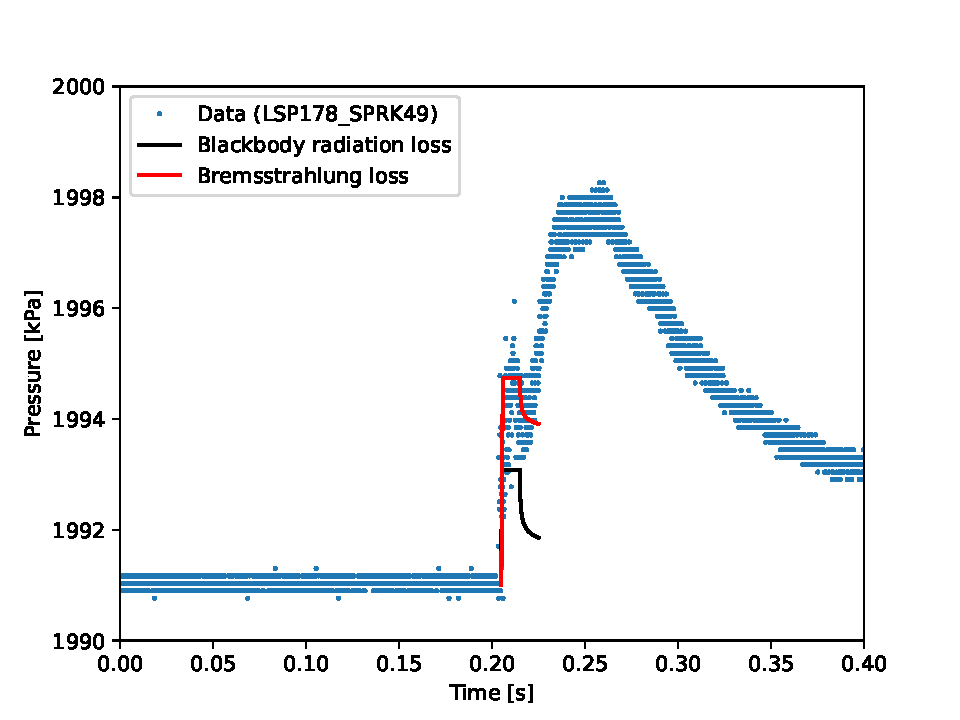
\includegraphics[width=0.85\textwidth]{assets/2 models/LSP178_SPRK49.pdf}
            \caption{Experimental data compared to the 0D model, with both Bremsstrahlung and blackbody losses}
            \label{fig:LSP178_SPRK49}
        \end{figure}
        
        Using Bremsstrahlung loss, the model appropriately approximated the first peak seen in the experimental data. Once the gas cooled down enough and stopped being ionized, Bremss-trahlung loss also stopped. The LSP cone in the model was then stable at approximately a temperature of \qty{5200}{K} and a pressure of \qty{2.003}{MPa}. As expected, the pressure rise was lower with blackbody radiation, as the loss was greater.

        Further investigation has shown that the model was not as sensitive as the experiments to a decrease in laser power, as can be seen in \autoref{fig:Two further LSPs}.

        \begin{figure}[!ht]
            \centering
            \begin{subfigure}[t]{0.45\textwidth}
                \centering
                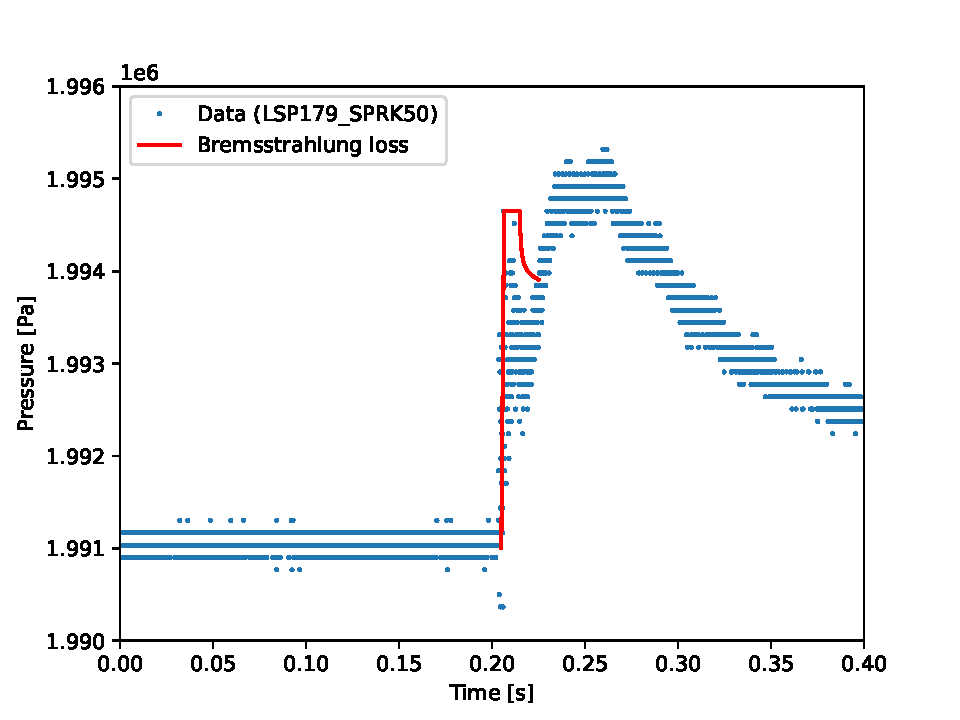
\includegraphics[width=\textwidth]{assets/2 models/LSP179_SPRK50.pdf}
                \caption{LSP179\_SPRK50, \qty{1540}{W} (50\% power) and initial pressure of \qty{19.91}{bar}}
            \end{subfigure}
            \hfill
            \begin{subfigure}[t]{0.45\textwidth}
                \centering
                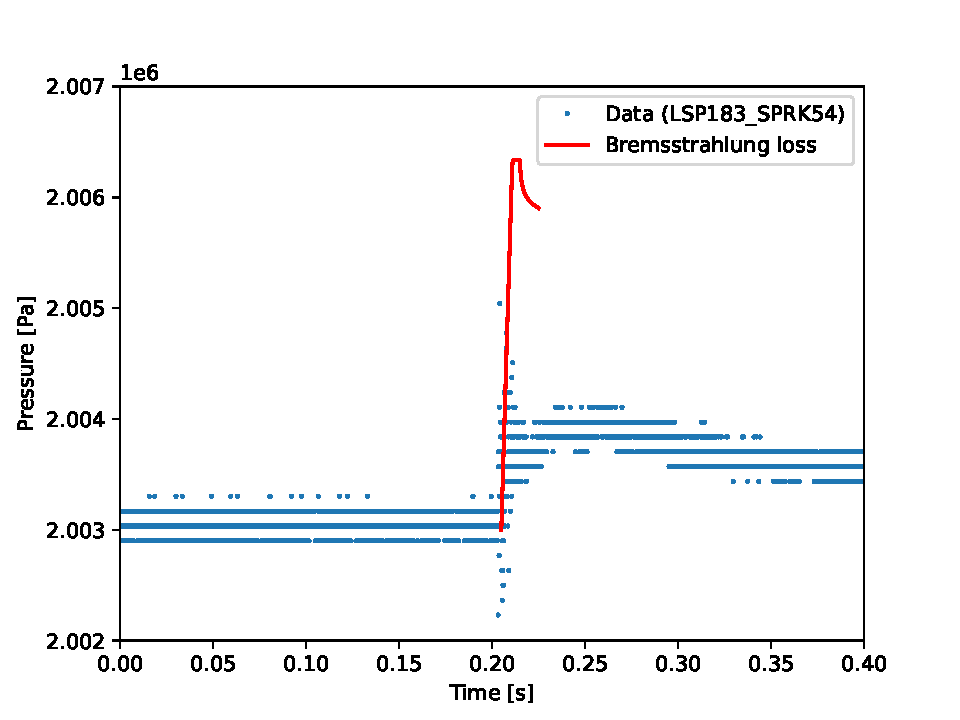
\includegraphics[width=\textwidth]{assets/2 models/LSP183_SPRK54.pdf}
                \caption{LSP183\_SPRK54, \qty{345}{W} (15\% power) and initial pressure of \qty{20.03}{bar}}
            \end{subfigure}
            \caption{Pressure change over time during two further LSPs, with Bremsstrahlung loss}
            \label{fig:Two further LSPs}
        \end{figure}

        Finally, \autoref{fig:powerVSdeltaP} shows how the pressure rise increased as the laser power was increased.

        \begin{figure}[!ht]
            \centering
            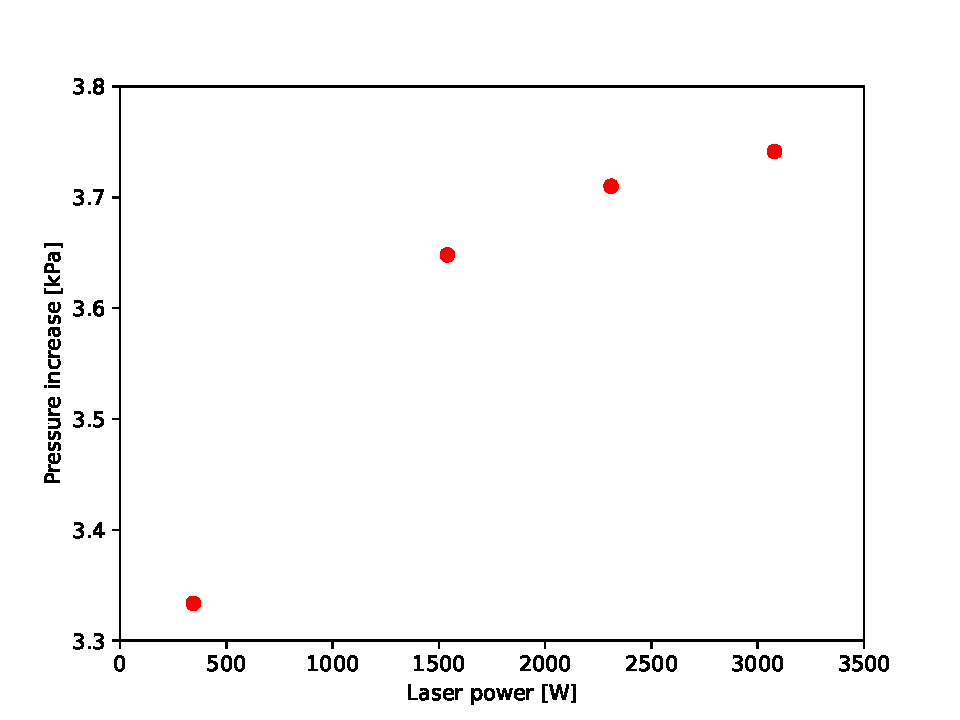
\includegraphics[width=0.85\textwidth]{assets/2 models/powerVSdeltaP.pdf}
            \caption{Pressure increase from 0D model as a function of laser power, with initial pressure of \qty{20}{bar}}
            \label{fig:powerVSdeltaP}
        \end{figure}

        For reference, \autoref{tab:Initial values for model} contains the initial values of each model run used for \autoref{fig:powerVSdeltaP}. Each run took around \qty{15}{minutes} to compute on a laptop.

        \begin{table}[!ht]
            \centering
            \caption{Initial values for 0D model}
            \label{tab:Initial values for model}
            \begin{tabularx}{\textwidth}{@{}lX<{\raggedright}X<{\raggedright}X<{\raggedright}X<{\raggedright}X<{\raggedright}@{}}
            \toprule
            Shot ID & $P_\mathrm{laser}$ (\unit{W}) & $P_\mathrm{laser}$ (\unit{\%}) & $p_\mathrm{ini}$ (\unit{bar}) & Time step (\unit{s}) & Source of $P_\mathrm{laser}$ (\unit{W})\\ \midrule
            LSP176\_SPRK47 & 2310      &  75     &    19.91   &  $50\times 10^{-6}$ & Maximum power multiplied by \% \\ 
            LSP178\_SPRK49 & 3079      &  100    &    19.91   &  $10\times 10^{-6}$ & Maximum power\\
            LSP179\_SPRK50 & 1540      &  50     &    19.91   &  $10\times 10^{-6}$ & Maximum power multiplied by \% \\
            LSP183\_SPRK54 & 345       &  15     &    20.03   & $10\times 10^{-6}$  & Extrapolated from \autoref{tab:laser shot statistics}\\ 
            \bottomrule
            \end{tabularx}
        \end{table}